\subsubsection{Ansatzfunktionen}

Um verzerrungsfreie Starrkörperbewegungen sowie konstante Verzerrungszustände beschreiben zu können und dabei ein räumlich isotropes Verformungsverhalten zu approximieren, müssen die Ansatzfunktionen vollständig sein.
Für ein ebenes Dreieckselement bedeutet dies z.B.
\begin{align}
u(\xi,\eta) &= \underbrace{\underbrace{ a_1 + a_2 \xi + a_3 \eta}_{\text{3 Knoten Dreieck}} + a_4 \xi^2 + a_5 \eta^2 + a_6 \xi \eta}_{\text{6 Knoten Dreieck}} \; .
\end{align}
Hier sind für ein 3-Knoten-Dreieckselement alle linearen Terme enthalten, für ein 6-Knoten-Dreieckselement sind auch die quadratischen und bilinearen Terme enthalten.
Illustriert kann man sich am besten ein pascalsches Dreieck wie in Abbildung Figure~\ref{pascaltriangle} vorstellen.

\begin{figure}[!htbp]
\centering
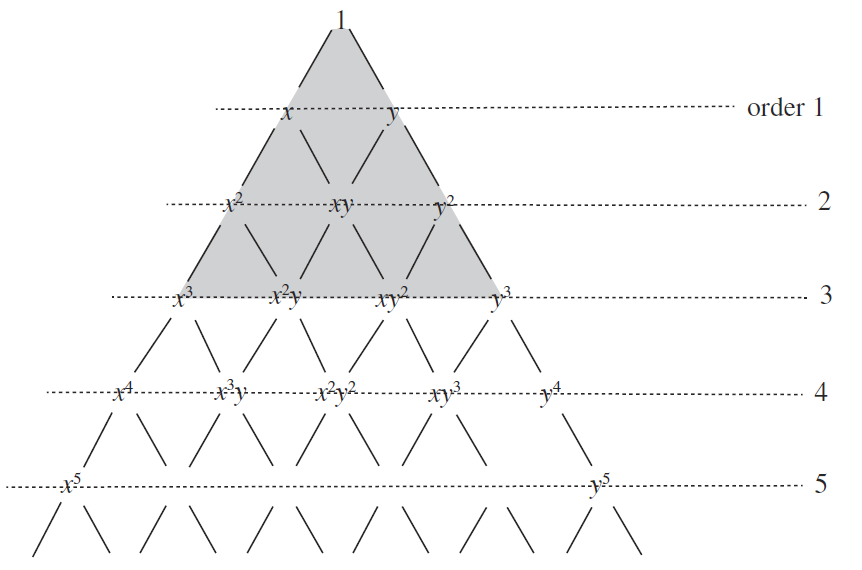
\includegraphics[width=0.45\linewidth]{files/Taylor_PascalTriangl-d58874fb2e0793428871a0933d31951f.png}
\caption[]{Pascal'sches Dreieck für Dreieckselemente (\cite{zienkiewicz2005finite})}
\label{pascaltriangle}
\end{figure}

Analog kann dazu ein vollständiges Viereckselement definiert werden:
\begin{align}
u(\xi,\eta) &= \underbrace{\underbrace{ a_1 + a_2 \xi + a_3 \eta + a_4 \xi \eta}_{\text{4 Knoten Viereck}} + a_5 \xi^2 + a_6 \eta^2 + a_7 \xi^2 \eta + a_8 \xi \eta^2}_{\text{8 Knoten Viereck}} \; .
\end{align}

Auch hier liefert das Pascalsche Dreieck eine anschauliche Interpretation:

\begin{figure}[!htbp]
\centering
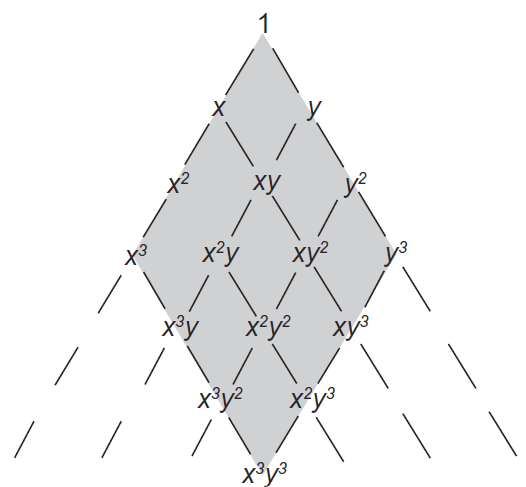
\includegraphics[width=0.45\linewidth]{files/Taylor_PascalQuad-53f0990e72ee0826eb02b4d26ee4606a.png}
\caption[]{Pascalsches Dreieck für Rechteckelemente (\cite{zienkiewicz2005finite}). Grau unterlegt ist ein kubisches Rechteckelement.}
\label{pascalQuad}
\end{figure}

\paragraph{Formfunktionen für $C^0$-Elemente}

Nachfolgend werden kurz die Ansatzfunktionen für 1D-, 2D- und 3D-Elemente mit Lagrange-Polynomen vorgestellt:

\subparagraph{1D Formfunktionen}

\begin{figure}[!htbp]
\centering
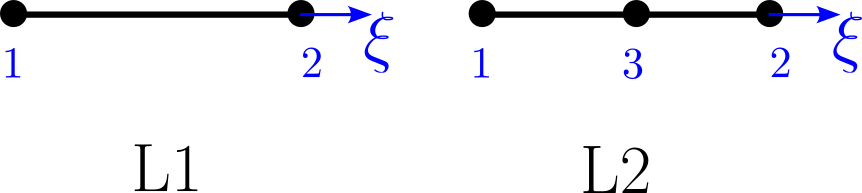
\includegraphics[width=0.625\linewidth]{files/Line-Elements-e2d4de7bd279c40b8dc47f1c98a894a5.png}
\caption[]{1D-Elemente mit linearer und quadratischer Ansatzfunktion}
\label{linearElements}
\end{figure}

Für den linearen Fall haben 1D-Elemente 2 Knoten und damit 2 Formfunktionen:

\begin{align}
N_1 &= \frac{1}{2} (1 - \xi) & N_2 &= \frac{1}{2} (1 + \xi)
\end{align}

Für den quadratischen Fall haben 1D-Elemente 3 Knoten und damit 3 Formfunktionen:
\begin{align}
N_1 &= \frac{1}{2} \xi (\xi - 1) & N_2 &= 1 - \xi^2 & N_3 &= \frac{1}{2} \xi (\xi + 1)
\end{align}

%  ```{figure} images/Shapefunctions_1d.png
% ---
% name: Shapefunctions_1dd
% alt: Formfunktionen für 1D-Elemente
% width: 500px
% ---
% Formfunktionen für 1D-Elemente
% ```

\subparagraph{2D Formfunktionen}

\begin{figure}[!htbp]
\centering
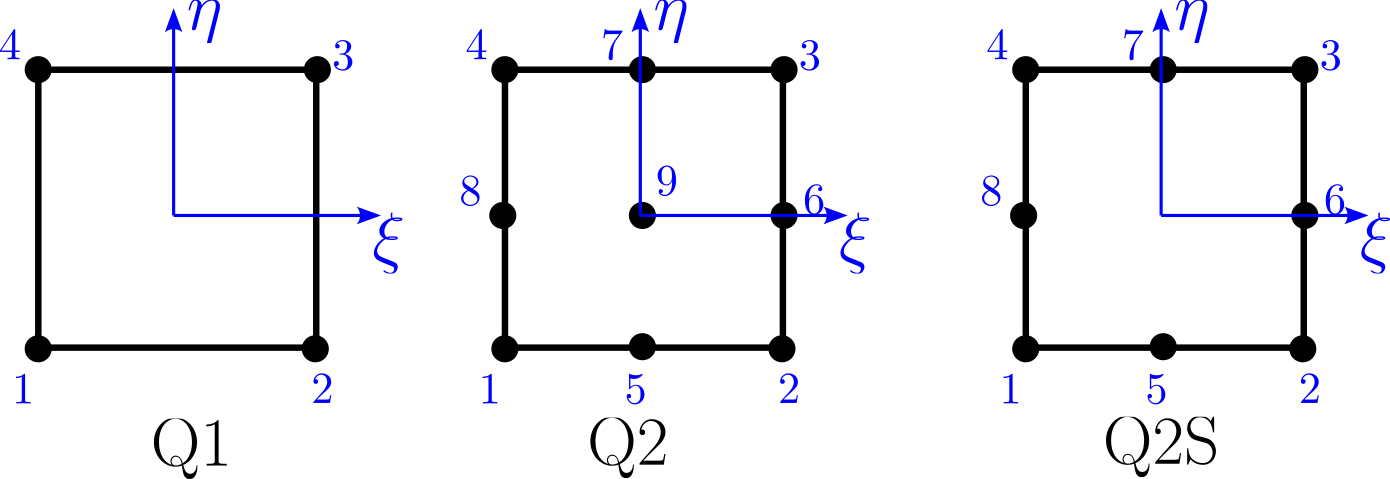
\includegraphics[width=0.625\linewidth]{files/QuadElements-3c42e67cc9a797973b3fd3afce627f44.png}
\caption[]{2D-Rechteck-Elemente mit linearer und quadratischer Ansatzfunktion}
\label{quadElements}
\end{figure}

Im 2D-Fall werden die Formfunktionen für Rechteck-Elemente als Tensorprodukt der 1D-Formfunktionen definiert. Für ein 2D-Rechteck-Element mit 4 Knoten (lineares Element) sind die Formfunktionen:

\begin{align}
N_1 &= \frac{1}{4} (1 - \xi)(1 - \eta) & N_2 &= \frac{1}{4} (1 + \xi)(1 - \eta) \\
N_3 &= \frac{1}{4} (1 + \xi)(1 + \eta) & N_4 &= \frac{1}{4} (1 - \xi)(1 + \eta)
\end{align}

\begin{figure}[!htbp]
\centering
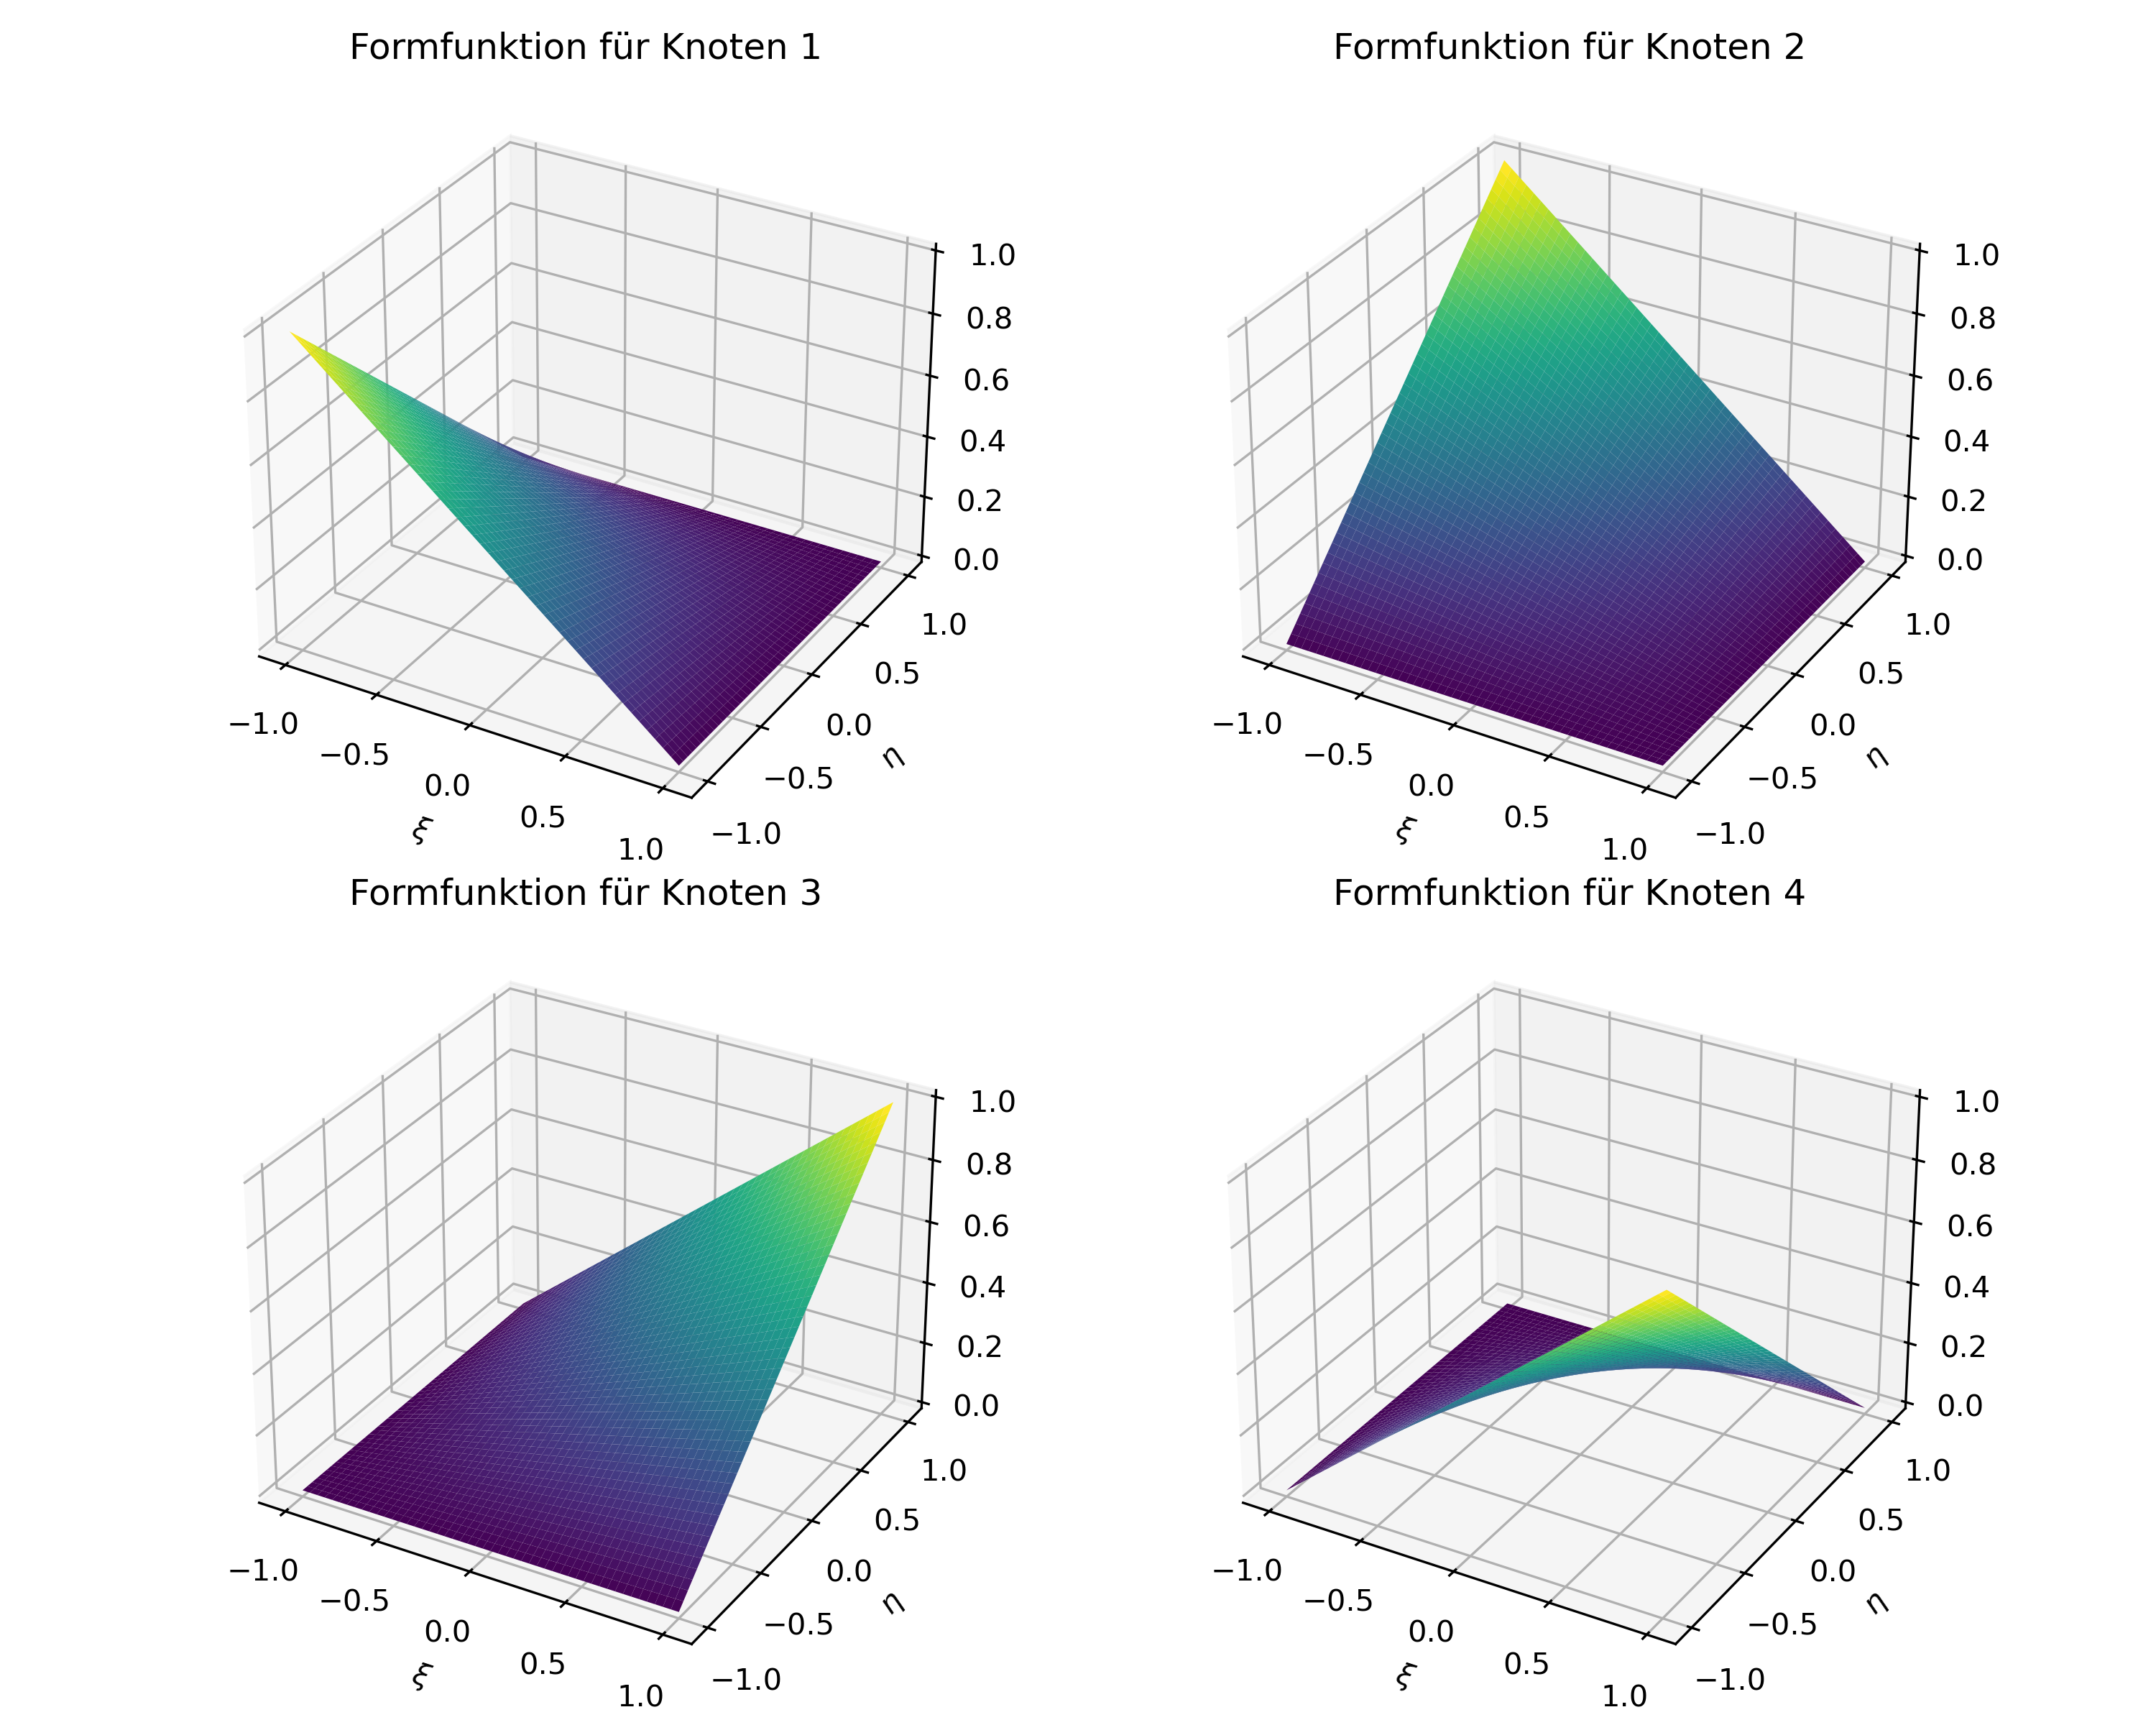
\includegraphics[width=0.625\linewidth]{files/shape_functions_Q4-1dbb3a2b8195bdb03c9a69d2f5a12df5.png}
\caption[]{Bilineare Formfunktionen für 2D-Rechteck-Elemente.}
\label{quadElementsQ4N}
\end{figure}

Um ein vollständiges Element der Ordnung 2 zu erhalten, benötigt man 9 Knoten beim Rechteck-Element. Die entsprechenden Formfunktionen lauten:

\begin{align*}
N_1 &= \frac{1}{4} \xi \eta (\xi - 1)(\eta - 1) & N_2 &= \frac{1}{2} (1 - \xi^2) (1 - \eta) \\
N_3 &= \frac{1}{4} \xi \eta (\xi + 1)(\eta - 1) & N_4 &= \frac{1}{2} (1 + \xi) (1 - \eta^2) \\
N_5 &= \frac{1}{4} \xi \eta (\xi + 1)(\eta + 1) & N_6 &= \frac{1}{2} (1 - \xi^2) (1 + \eta) \\
N_7 &= \frac{1}{4} \xi \eta (\xi - 1)(\eta + 1) & N_8 &= \frac{1}{2} (1 - \xi) (1 - \eta^2) \\
N_9 &= (1 - \xi^2)(1 - \eta^2)
\end{align*}

\begin{figure}[!htbp]
\centering
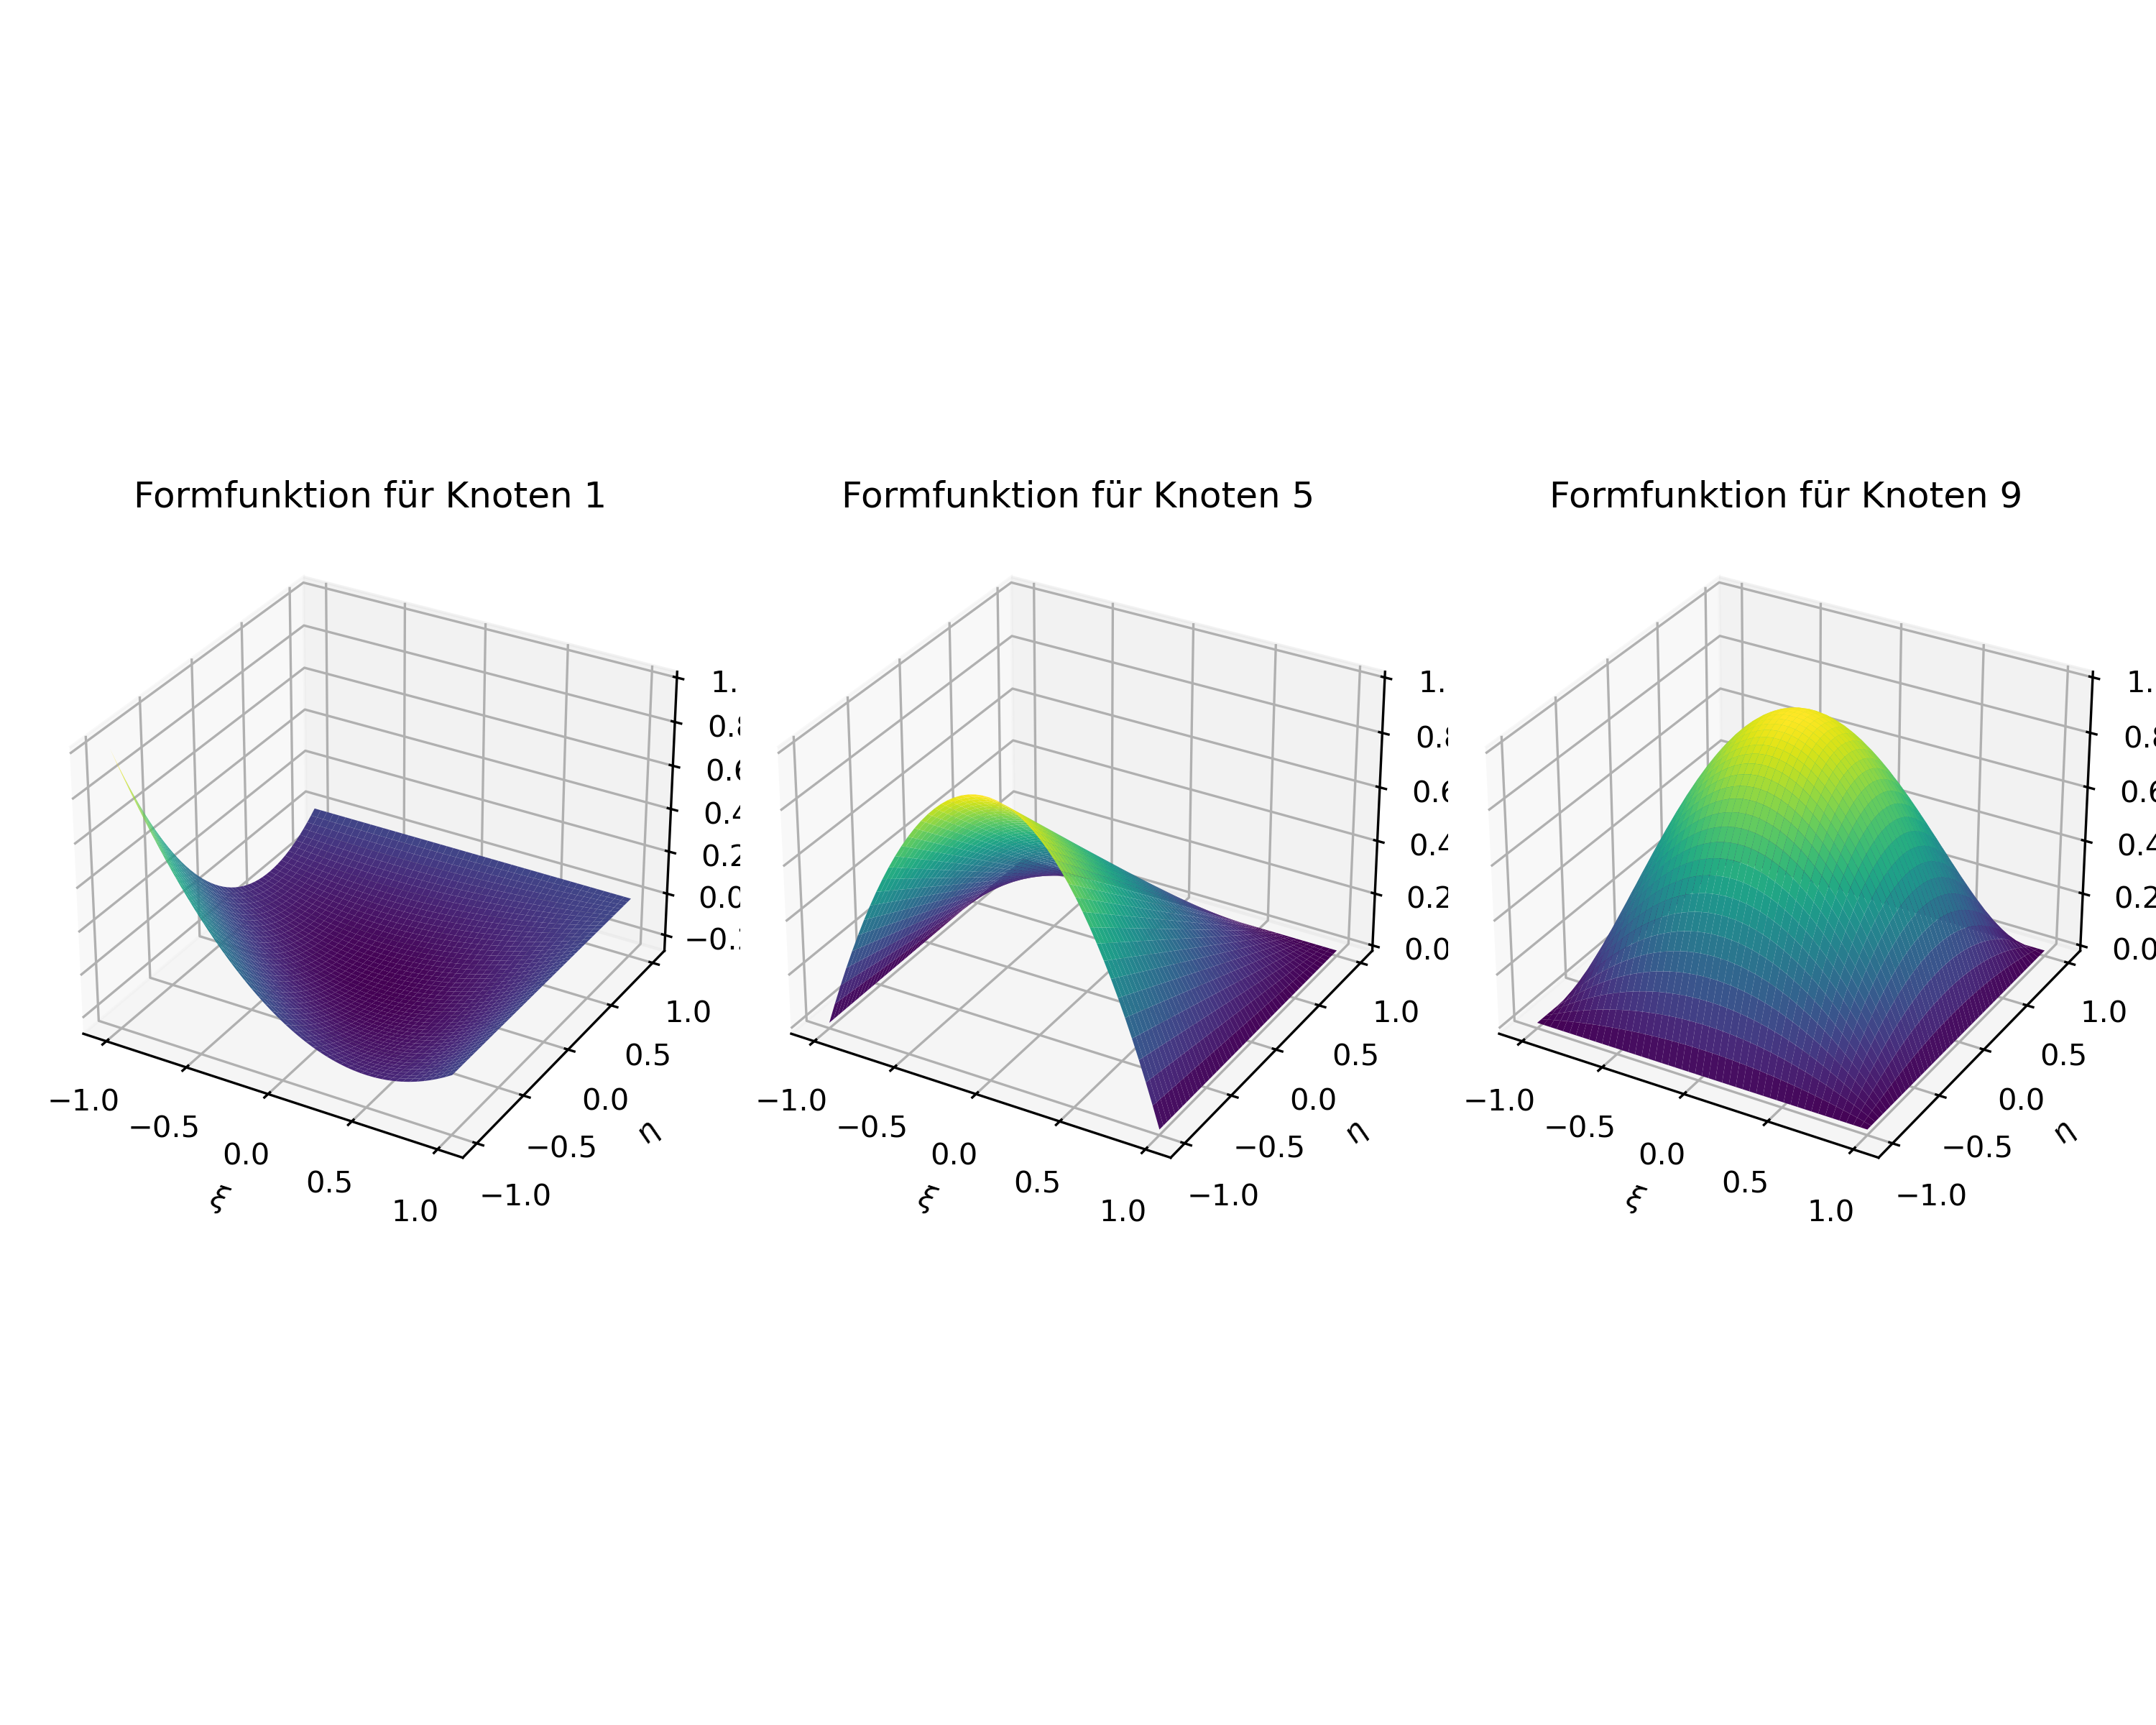
\includegraphics[width=0.625\linewidth]{files/shape_functions_Q9-4b92558abd04628eb843f07d85382fbd.png}
\caption[]{Biquadratische Formfunktionen für 2D-Rechteck-Elemente (Q2).}
\label{quadElementsQ9N}
\end{figure}

In der Praxis der Finite-Elemente-Methode beschränkt man sich jedoch nicht ausschlie$\beta$lich auf Q9-Elemente, die die vollständige Polynomordnung 2 aufweisen, wie in Abbildung Figure~\ref{pascalQuad} dargestellt. Serendipity-Elemente sind im oben beschriebenen Sinne nicht vollständig, erfüllen jedoch die Anforderungen an die räumliche Isotropie, die Verzerrungsfreiheit bei Starrkörperbewegungen und die Abbildung konstanter Verzerrungszustände. Der Begriff „Serendipity`` geht vermutlich auf ein Märchen von H. Walpole, „Die drei Prinzen von Serendip``, zurück, in dem die Prinzen die Fähigkeit besitzen, durch Zufall unverhoffte und glückliche Entdeckungen zu machen. Das zugehörige Element ist in Abbildung Figure~\ref{quadElements} als \textbf{Q2S} dargestellt. Die Ansatzfunktionen lauten:

\begin{align}
N_1(\xi ,\eta ) & =\frac{1}{4} (1-\eta ) (1-\xi ) (-\eta -\xi -1) & N_2(\xi ,\eta ) & =\frac{1}{4} (1-\eta ) (\xi +1) (-\eta +\xi -1) \\
N_3(\xi ,\eta ) & =\frac{1}{4} (\eta +1) (\xi +1) (\eta +\xi -1) & N_4(\xi ,\eta ) & =\frac{1}{4} (\eta +1) (1-\xi ) (\eta -\xi -1) \\
N_5(\xi ,\eta ) & =\frac{1}{2} (1-\eta ) \left(1-\xi ^2\right) & N_6(\xi ,\eta ) & =\frac{1}{2} \left(1-\eta ^2\right) (\xi +1)\\
N_7(\xi ,\eta ) & =\frac{1}{2} (\eta +1) \left(1-\xi ^2\right) &
N_8(\xi ,\eta ) & =\frac{1}{2} \left(1-\eta ^2\right) (1-\xi )
\end{align}

\begin{figure}[!htbp]
\centering
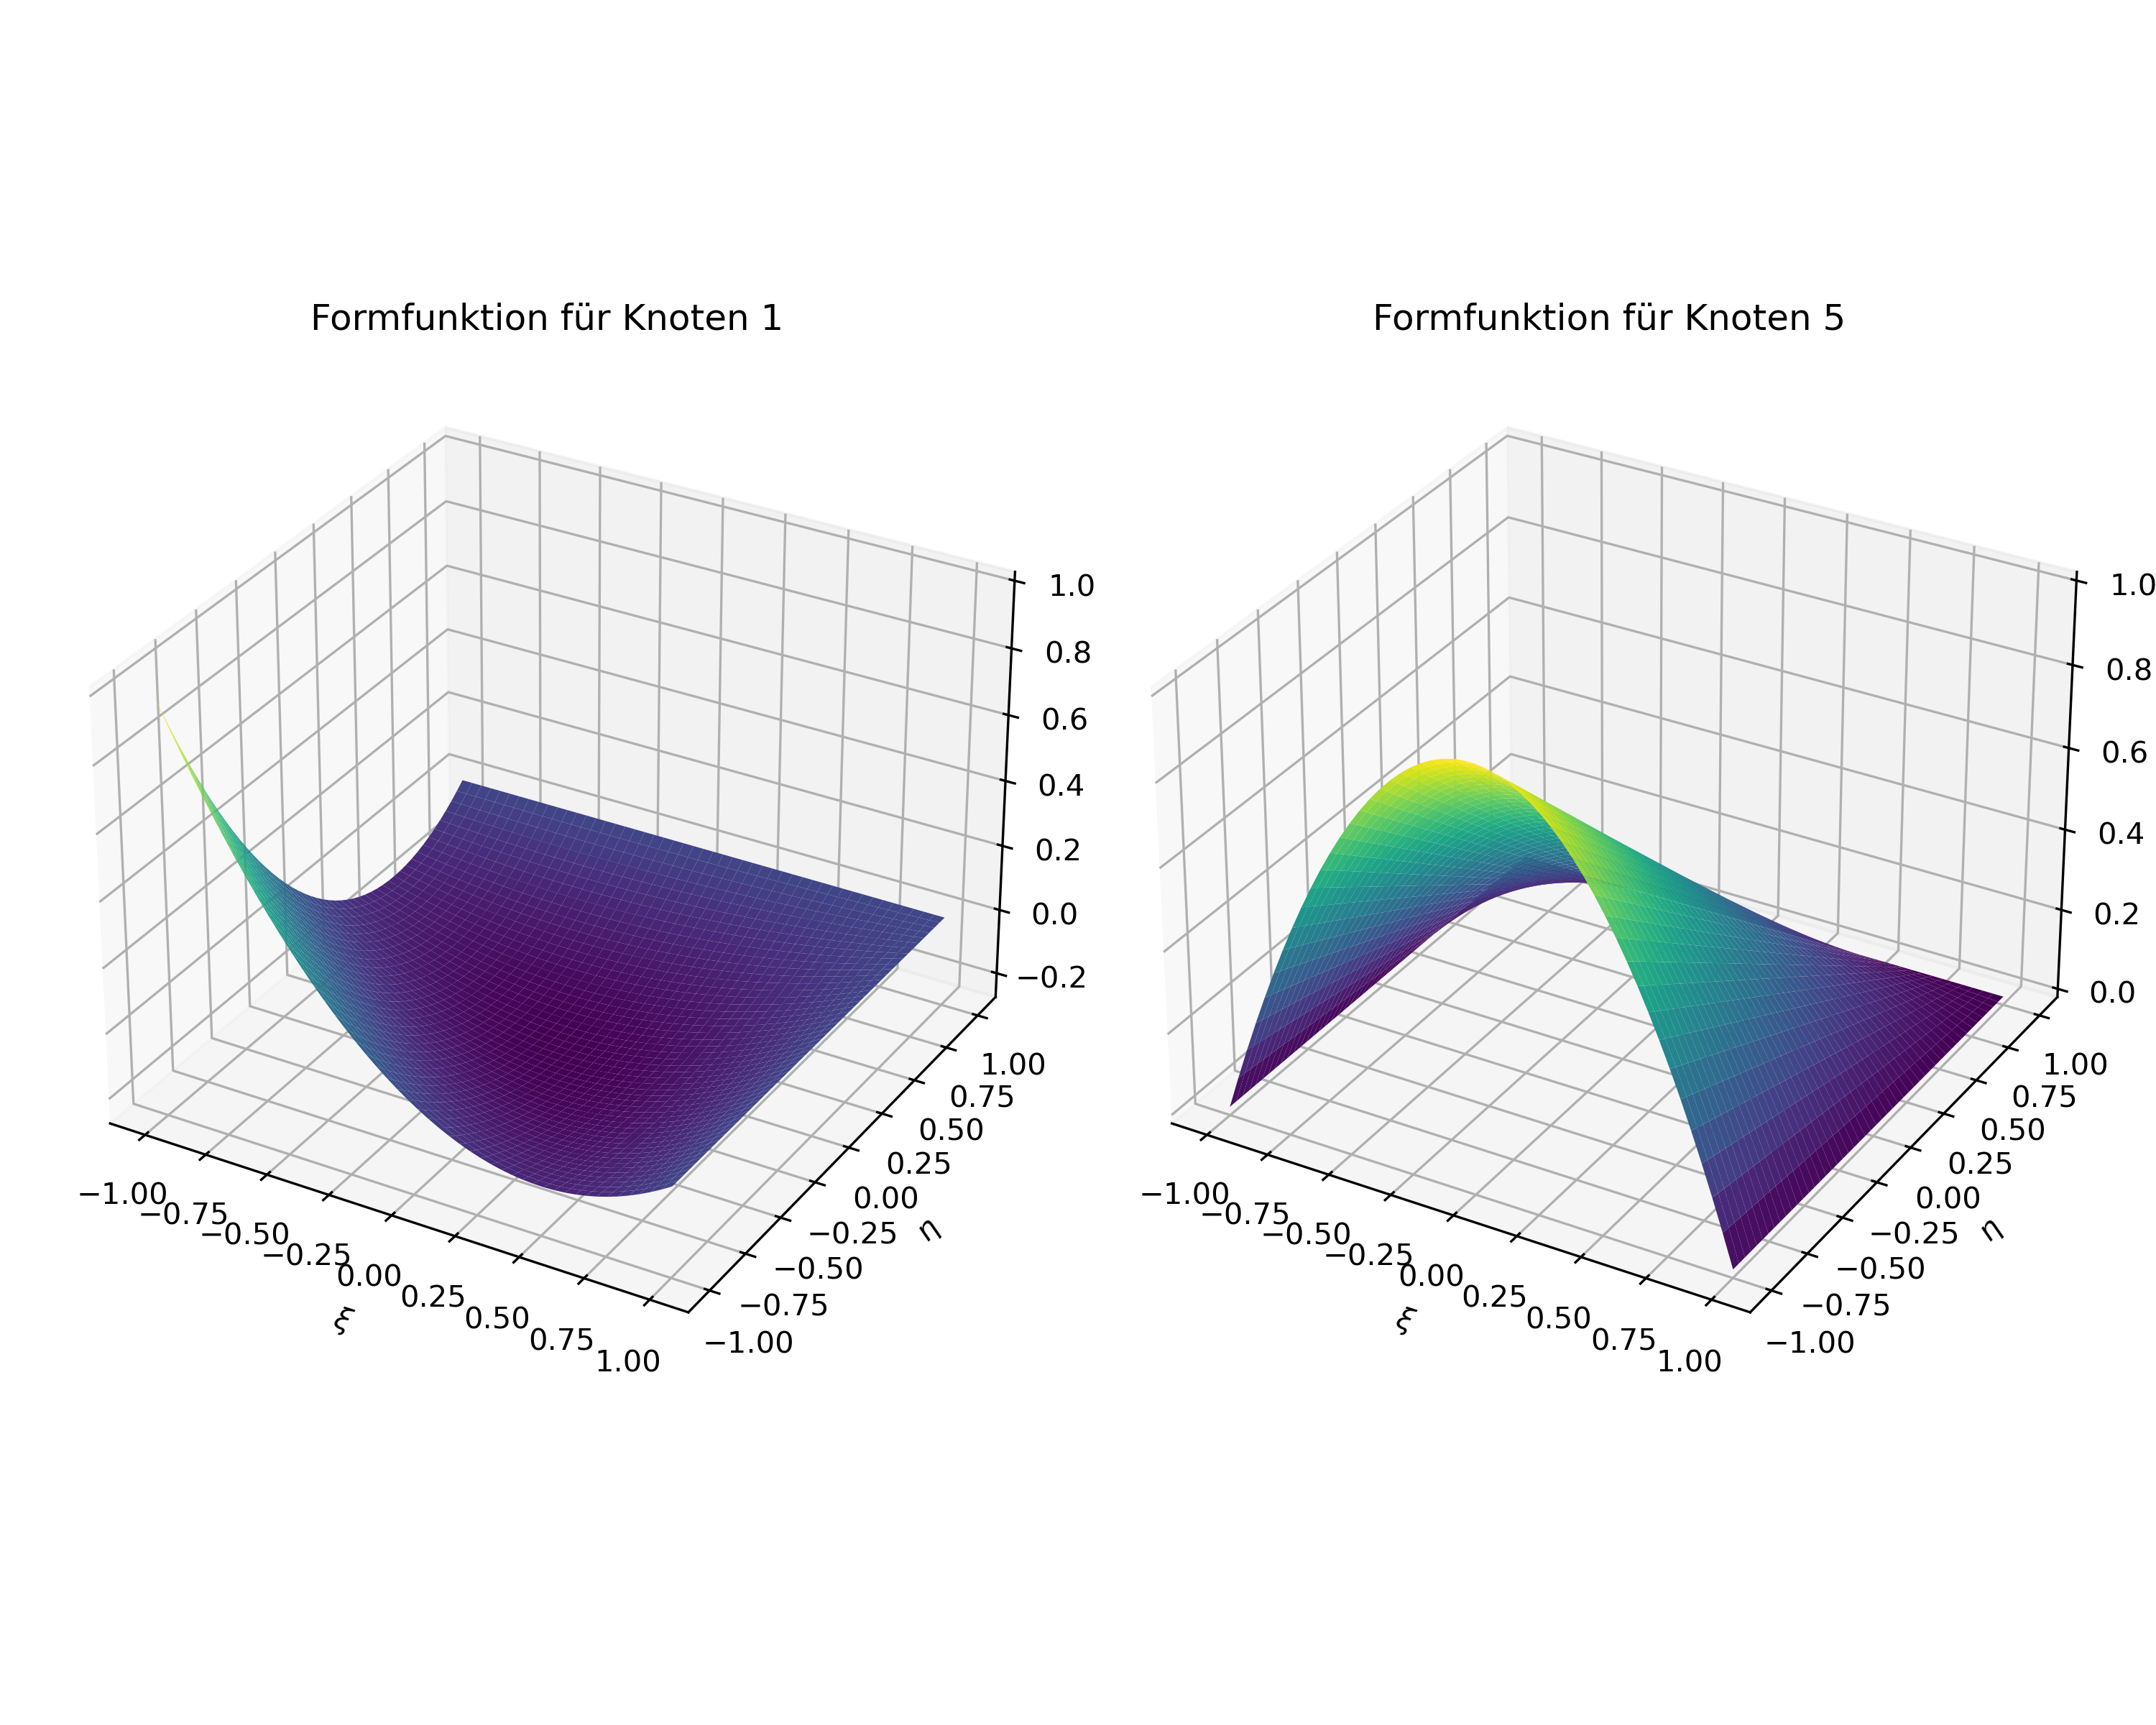
\includegraphics[width=0.625\linewidth]{files/shape_functions_Q8-48d9fa7e53fa8fe13e232d8a4fc0aa98.png}
\caption[]{Biquadratische Serendipity-Formfunktionen für 2D-Rechteck-Elemente (Q2S).}
\label{quadElementsQ8N}
\end{figure}

Eine weitere Möglichkeit der zweidimensionalen Vernetzung ist die Verwendung von Dreiecken. In den gebräuchlichen FEM-Programmen werden dabei Dreiecke mit 3 oder 6 Knoten implementiert. Diese sind in Figure~\ref{triangleElements} dargestellt.

\begin{figure}[!htbp]
\centering
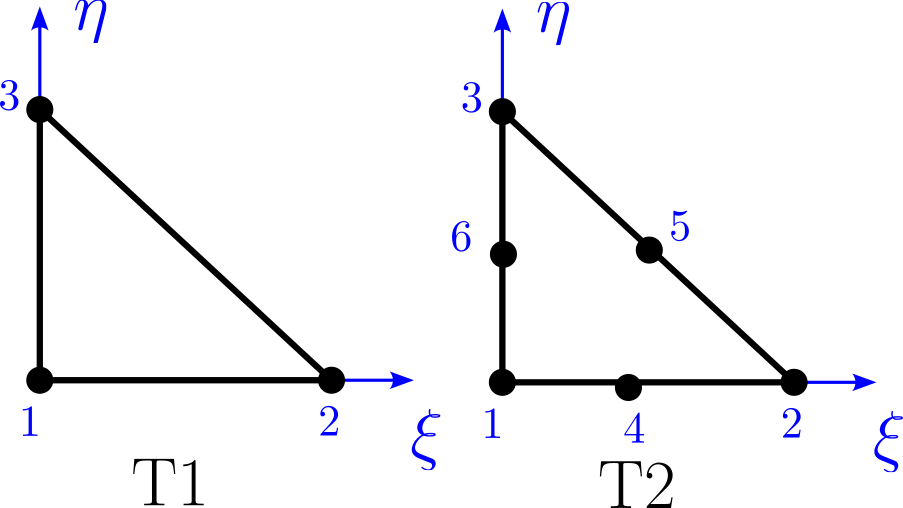
\includegraphics[width=0.625\linewidth]{files/TriangleElements-0c3b6af2501f4575008c6e8b2ea02f48.png}
\caption[]{Dreieck-Elemente mit linearen (T1) und quadratischen (T2) Formfunktionen.}
\label{triangleElements}
\end{figure}

Die linearen Dreieck-Elemente (T1) sind die einfachsten Elemente und werden in der Literatur häufig als ``konstant'' bezeichnet. Dies bezieht sich auf die abgeleiteten Grö$\beta$en (z.B. Spannungen, Dehnungen, etc.), die als konstant dargestellt werden. Die Formfunktionen lauten:

\begin{align}
\lambda & = 1 - \xi - \eta & N_1(\xi ,\eta ) & = \lambda \\
N_2(\xi ,\eta ) & = \xi & N_3(\xi ,\eta ) & = \eta
\end{align}

\begin{figure}[!htbp]
\centering
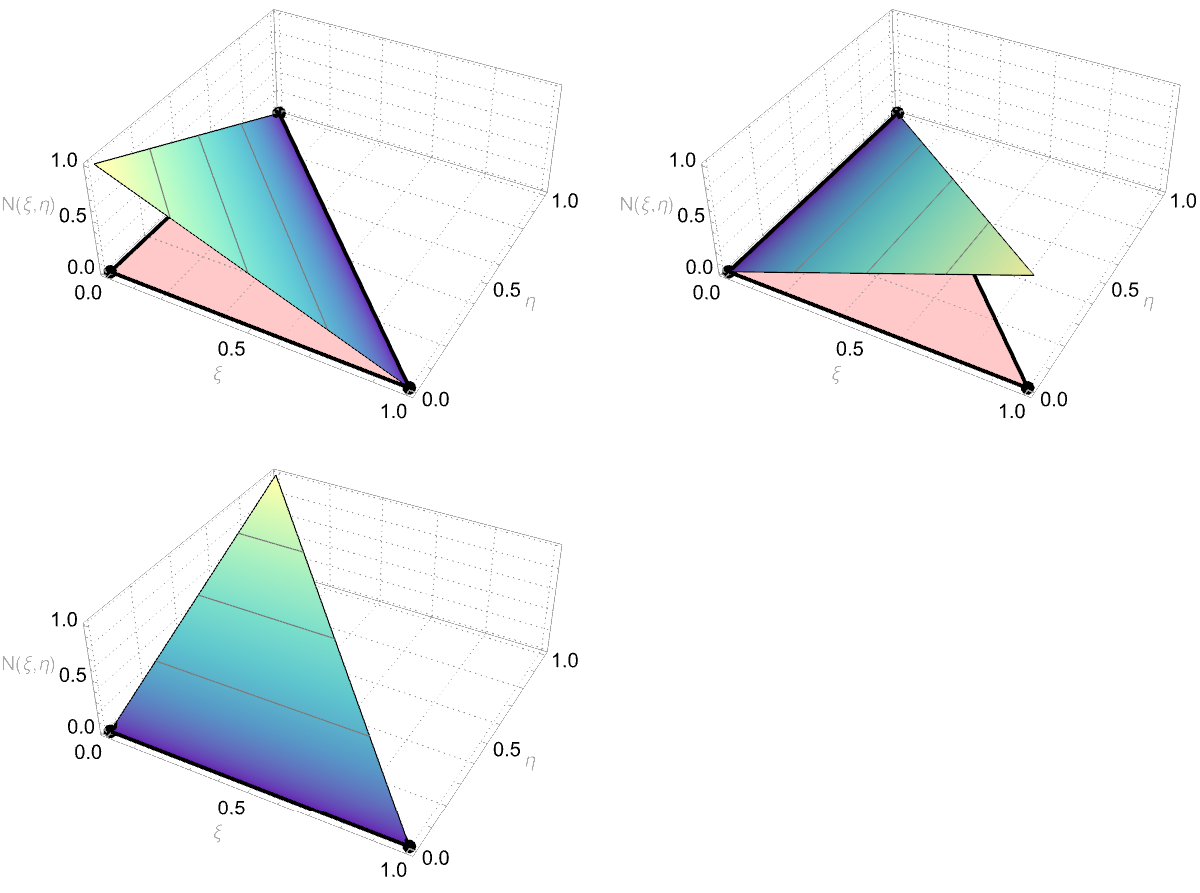
\includegraphics[width=0.625\linewidth]{files/shape_T1-594d407f8c44ecc83abb40efc728a385.png}
\caption[]{Formfunktionen für das Dreieck-Element T1.}
\label{shapefunTria}
\end{figure}

Die Formfunktionen für Dreieck-Elemente mit 6 Knoten (T2) sind vollständig quadratisch. Insgesamt hat das T2-Element bessere Approximationseigenschaften als das T1-Element. Die Formfunktionen lauten:

\begin{align}
\lambda & = 1 - \xi - \eta & N_1(\xi ,\eta ) & = \lambda (2\lambda - 1) \\
N_2(\xi ,\eta ) & = \xi (2\xi - 1) & N_3(\xi ,\eta ) & = \eta (2\eta - 1) \\
N_4(\xi ,\eta ) & = 4\lambda \xi & N_5(\xi ,\eta ) & = 4\xi \eta \\
N_6(\xi ,\eta ) & = 4\lambda \eta
\end{align}

\subparagraph{3D Formfunktionen}

\begin{figure}[!htbp]
\centering
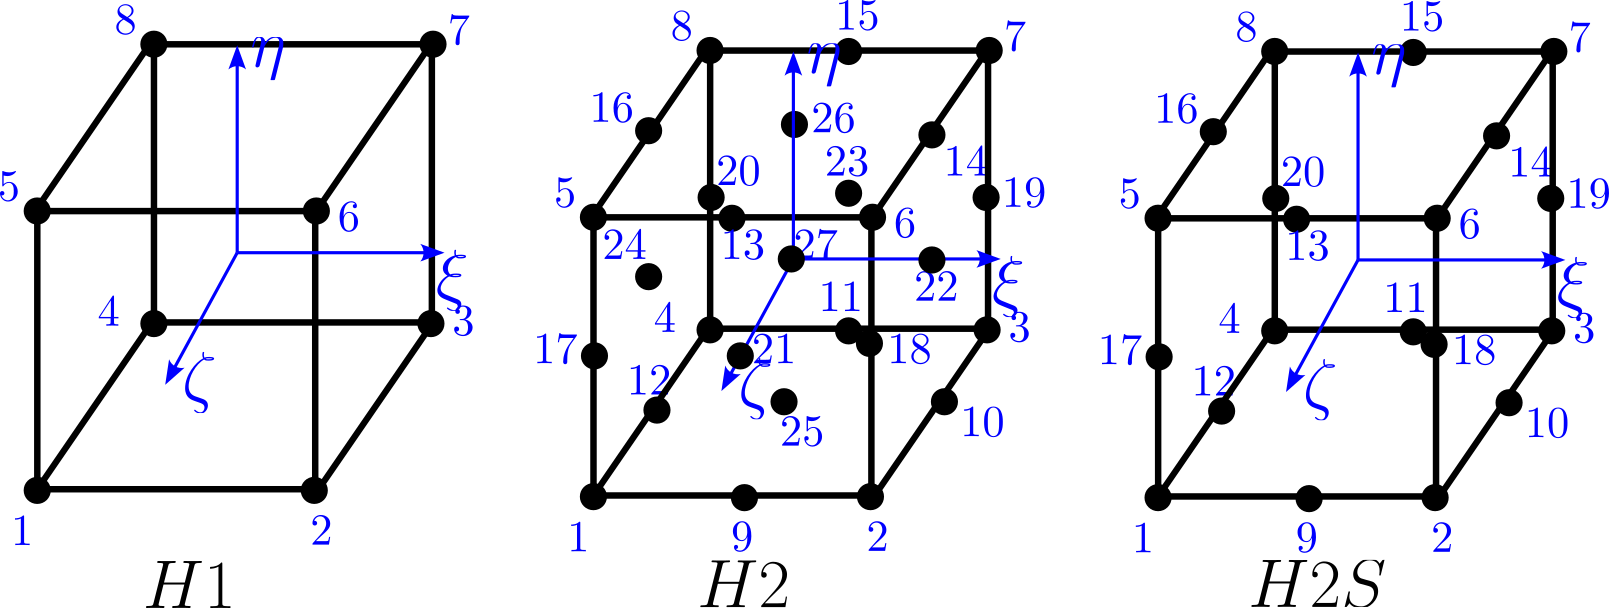
\includegraphics[width=0.625\linewidth]{files/HexElements-a4ee848a8b573d56dbd74d399701e925.png}
\caption[]{3D-Hexaeder-Elemente mit linearer (8 Knoten) und quadratischer (27 Knoten) Approximation. Zusätzlich ist das 20-Knoten-Hexaeder-Serendipity-Element gezeigt.}
\label{hexElements}
\end{figure}

Im 3D-Fall werden die Formfunktionen für Hexaeder-Elemente als Tensorprodukt der 1D-Formfunktionen definiert. Für ein 3D-Hexaeder-Element mit 8 Knoten (lineares Element) sind die Formfunktionen:

\begin{align}
N_1 &= \frac{1}{8} (1 - \xi)(1 - \eta)(1 - \zeta) & N_2 &= \frac{1}{8} (1 + \xi)(1 - \eta)(1 - \zeta) \\
N_3 &= \frac{1}{8} (1 + \xi)(1 + \eta)(1 - \zeta) & N_4 &= \frac{1}{8} (1 - \xi)(1 + \eta)(1 - \zeta) \\
N_5 &= \frac{1}{8} (1 - \xi)(1 - \eta)(1 + \zeta) & N_6 &= \frac{1}{8} (1 + \xi)(1 - \eta)(1 + \zeta) \\
N_7 &= \frac{1}{8} (1 + \xi)(1 + \eta)(1 + \zeta) & N_8 &= \frac{1}{8} (1 - \xi)(1 + \eta)(1 + \zeta)
\end{align}

Um ein vollständiges Element der Ordnung 2 zu erhalten, benötigt man 27 Knoten beim Hexaeder-Element. Die Formfunktionen kann man zum Beispiel \cite{wriggers2008nonlinear} entnehmen. Mehr Verwendung findet das 20-Knoten-Element. Hierbei handelt es sich um ein Serendipity-Element, das nicht vollständig von der Ordnung 2 ist, aber die Bedingungen der Raumisotropie, keine Verformung bei starren Körperbewegungen und die Möglichkeit, konstante Spannungszustände zu modellieren, erfüllt.

Für tetraedrische Elemente implementieren gängige FEM-Programme Tetraeder mit entweder 4 oder 10 Knoten. Diese sind in Abbildung Figure~\ref{tetraElements} dargestellt.

\begin{figure}[!htbp]
\centering
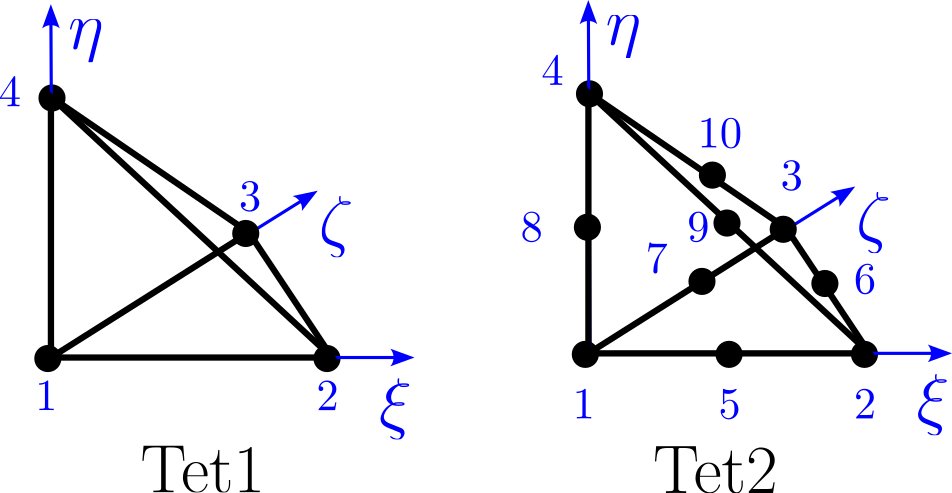
\includegraphics[width=0.625\linewidth]{files/TetElements-996ee625624fda771512d85c968c03fc.png}
\caption[]{Tetraedrische Elemente mit linearen (Tet1) und quadratischen (Tet2) Formfunktionen.}
\label{tetraElements}
\end{figure}

Die linearen Tetraederelemente (T4) sind die einfachsten und werden häufig als ``konstante'' Elemente in der Literatur bezeichnet, wobei sich dies auf die abgeleiteten Grö$\beta$en (z.B. Spannungen, Dehnungen, etc.) bezieht. Die Formfunktionen lauten:

\begin{align}
\lambda &= 1 - \xi - \eta - \zeta & N_1(\xi ,\eta ,\zeta ) &= \lambda \\
N_2(\xi ,\eta ,\zeta ) &= \xi & N_3(\xi ,\eta ,\zeta ) &= \eta & N_4(\xi ,\eta ,\zeta ) &= \zeta
\end{align}

Die Formfunktionen für tetraedrische Elemente mit 10 Knoten (T10) sind vollständig quadratisch und bieten bessere Approximationseigenschaften als das T4-Element. Die Formfunktionen lauten:

\begin{align}
\lambda &= 1 - \xi - \eta - \zeta & N_1(\xi ,\eta ,\zeta ) &= \lambda (2\lambda - 1) \\
N_2(\xi ,\eta ,\zeta ) &= \xi (2\xi - 1) & N_3(\xi ,\eta ,\zeta ) &= \eta (2\eta - 1) \\
N_4(\xi ,\eta ,\zeta ) &= \zeta (2\zeta - 1) & N_5(\xi ,\eta ,\zeta ) &= 4\lambda \xi \\
N_6(\xi ,\eta ,\zeta ) &= 4\xi \eta & N_7(\xi ,\eta ,\zeta ) &= 4\lambda \eta \\
N_8(\xi ,\eta ,\zeta ) &= 4\lambda \zeta & N_9(\xi ,\eta ,\zeta ) &= 4\xi \zeta \\
N_{10}(\xi ,\eta ,\zeta ) &= 4\eta \zeta
\end{align}

\begin{framed}
\textbf{Fragen zum Kapitel}\\
\textbf{Ansatzfunktionen}

\begin{itemize}
\item Wieviele Knoten hat ein Tetraeder-Element mit linearen Ansatzfunktionen?
\item Wieviele Knoten hat ein Viereck-Element mit quadratischen Ansatzfunktionen?
\item Eine wichtige Eigenschaft der gezeigten Formfunktionen ist, dass sie nur am zugehörigen Knoten den Wert 1 annehmen. An allen anderen Knoten ist der Wert 0. Was bedeutet dies für den Knotenfreiheitsgrad bzgl. seiner physikalischen Deutbarkeit?
\item Welche Aussage ist richtig?\begin{itemize}
\item Bei Formfunktionen mit quadratischem Polynomgrad ist der Verlauf der Dehnungen im Element quadratisch.
\item Bei Formfunktionen mit linearem Verlauf sind die Verschiebungen im Element linear.
\item Die Dehnungen sind über die Elementränder hinweg stetig für Formfunktionen mit quadratischem Polynomgrad.
\item Die Summe der Ansatzfunktionen im Element ist stets 1.
\end{itemize}
\end{itemize}
\end{framed}